\chapter{Results}


\section{Multi-bed Dynamic Whole Body PET: Acquisition optimization}
\section{Introduction}
In PET imaging one of the needs in many clinical and research applications is acquisition of information over the whole body. Moreover, dynamic information over the whole body can allow for research applications of PET, such as in pharmacokinetics, to expand to the whole body and also allow for exploration of potential future clinical applications. 
An important limitation of DWB protocols in scanners with limited A-FOV is the result temporal gaps in the acquired data of any given bed position. These are introduced at each bed position by the time spent on imaging other bed positions and from the time required to move the bed to the next position and prepare for the next acquisition. 
In practice for scanners that have no in-build DWB protocol, such as the Signa PET/MR, a large fraction of the acquisition delays in DWB protocols are attributed to a greater extend to system processes that are lunched automatically between WB sweeps rather than to time taken to move the bed between bed positions. These processes include transfer of raw data files and reconstructions performed during scanning. More acquisition time could be gained if those could be avoided and delays were decreased.

In this chapter we review results of acquisition performance from a dynamic whole-body (DWB) protocol implemented on the Signa PET/MR scanner as part of the IsotoPK pharmacokinetic study~\cite{Marie2019}. A short introduction on the design of the protocol using current scanner features is given, with details on processing and exportation of the data provided in Appendix~\ref{chap:AppendixA}.
We then describe the implementation of an experimental fully-automated protocol for DWB acquisitions on the Signa PET/MR, that was designed with the aim of reducing acquisition delays and allow for greater flexibility in selection of bed positions. The development of this protocol was conducted as part of this project and in collaboration with GE Healthcare. 
Finally, we present results of the experimental acquisition protocol applied on a \gls{nhp} study and compare against the standard DWB protocol used in the IsotoPK study with data from fourteen volunteer scans.


\section{Design and Performance of a DWB protocol on the Signa PET-MR}
Prior to commencing this PhD project and in perpetration for the IsotoPK study, a DWB protocol was designed on the GE Signa PET/MR scanner. The desired coverage was achieved using 5 bed positions and a reduced overlap, as shown in diagram (C) of figure~\ref{fig3_1:BodyCoverage}. The relatively small overlap (half compared to routine clinical protocols) was selected to reduce the number of beds and subsequently the acquisition temporal gaps.
The study design was limited to a total duration of 1 hour from injection and includes an initial dynamic single-bed phase centred over the liver, where the highest expression of the transporters under study was expected. 
The single-bed dynamic position was imaged for 3 minutes from injection, prior to the start of DWB acquisition.
Because the system has no in-build protocols for DWB imaging, a custom protocol had to be made using a series of Static WB acquisition protocols. Each WB pass has to be individually pre-planned, which results in fixed bed positions (relevant to a reference mark for each volunteer). The volunteer positioning was made using a chest-landmark, but no further adjustments of the protocol were possible for optimum positioning of the bed positions, relative to each patient's size.

For the design of the framing used in the isotoPK DWB protocol, the following empirical metric has been taken under consideration. We define the Delays to Acquisition ratio (DAR) as the ratio of total delays to acquisition time for every WB sweep, using the relationship
\begin{equation} \label{eqn:acq_to_dead_time}
 \mathrm{DAR} = \frac{dl_{bed}\cdot 4 + dl_{Sweep}}{t_{duration}\cdot 5 }  \\ , \\ 
\end{equation}
where $t_{duration}$ is the frame duration for a single bed in the WB sweep, $dl_{bed}$ the delays between adjacent beds and $dl_{Sweep}$ the delay between WB sweeps.
First estimations of the delay times for the Signa PET-MR had shown a delay of approximately 6 seconds between adjacent bed positions and 20 seconds between WB sweeps. Using this information, the framing sequence shown in table~\ref{tab:IsotoPK_Framing} was chosen with the shortest frame duration set to 20 seconds in order to maintain a DAR greater than 50\% at the early phases of the DWB study. 

\begin{table}[]
\caption{Framing of IsotoPK DWB protocol.}
\label{tab:IsotoPK_Framing}
\begin{tabular}{|l|l|l|l|l|}
\toprule
\textbf{Phase ID} & \textbf{Description}              & \textbf{Frame Duration (s)} & \textbf{Nb Frames} & \textbf{delay to acq. ratio} \\
\midrule
1        & Single-Bed dynamic phase & 10                 & 18        & N/A                 \\
2        & DWB                      & 20                 & 9         & 44\%                \\
3        & DWB                      & 30                 & 8         & 29\%                \\
4        & DWB                      & 40                 & 2         & 22\%                \\
\bottomrule
\end{tabular}
\end{table}

MR sequences required for attenuation correction (MRACs) were performed prior and during the DWB protocol acquisition. The first MRAC sequence at each bed location lasted approximately 35 seconds, with subsequent scans over the same locations lasting approximately 21 seconds per bed. MRAC acquisitions were not repeated for all WB sweeps of the DWB protocol, to allow for entry in the room for acquisition of blood samples required for derivation of the input function and metabolite analysis. 
A details description of the steps and their naming is given in table~\ref{tab:IsotPK_CE_details} for each WB sweep. %(refereed in protocol naming as \textit{CE}, standing for whole body "corps entier" in French)

The acquired DWB data were initially reconstructed at the system console.
Then, as part of this PhD project, the raw data were retrospectively exported for offline processing and treated with the steps of an automated pipe-line described in Appendix~\ref{chap:AppendixA}.

\subsection{Results from IsotoPK study}

The result beds positions of the DWB protocol can be seen in figures~\ref{fig3_1:rif_mips} and ~\ref{fig3_1:ctrl_mips} for the fourteen studies of the IsotoPK protocol evaluated.
Using the timing information of the extracted raw PET data, the average delay times per imaged subject were estimated, shown in the form of box-plots for $dl_{bed}$ in figure~\ref{fig3_1:BoxPlots_beds} and for $dl_{Sweep}$ in figure~\ref{fig3_1:BoxPlots_sweeps}.

It is noteworthy that with accumulation of experience in performing the DWB protocol the delays between sweeps were reduced considerably, for the most recent examinations compared to the first. This can be attributed to improved preparation of the PET/MR system before performing the protocol (ex. reboot of the system prior to acquisition, etc.).
For the 3 more recent subject examinations the average intra-bed delay time $dl_{bed}$ was 5.69 s (95\%CI: 5.63,5.75) and the average delay time between sweeps $dl_{Sweep}$ was 26.17 s (95\%CI: 26.13, 26.22).
These values are close to the one considered in the design of the protocol.\\

%
\begin{figure} [ht!]
\centering
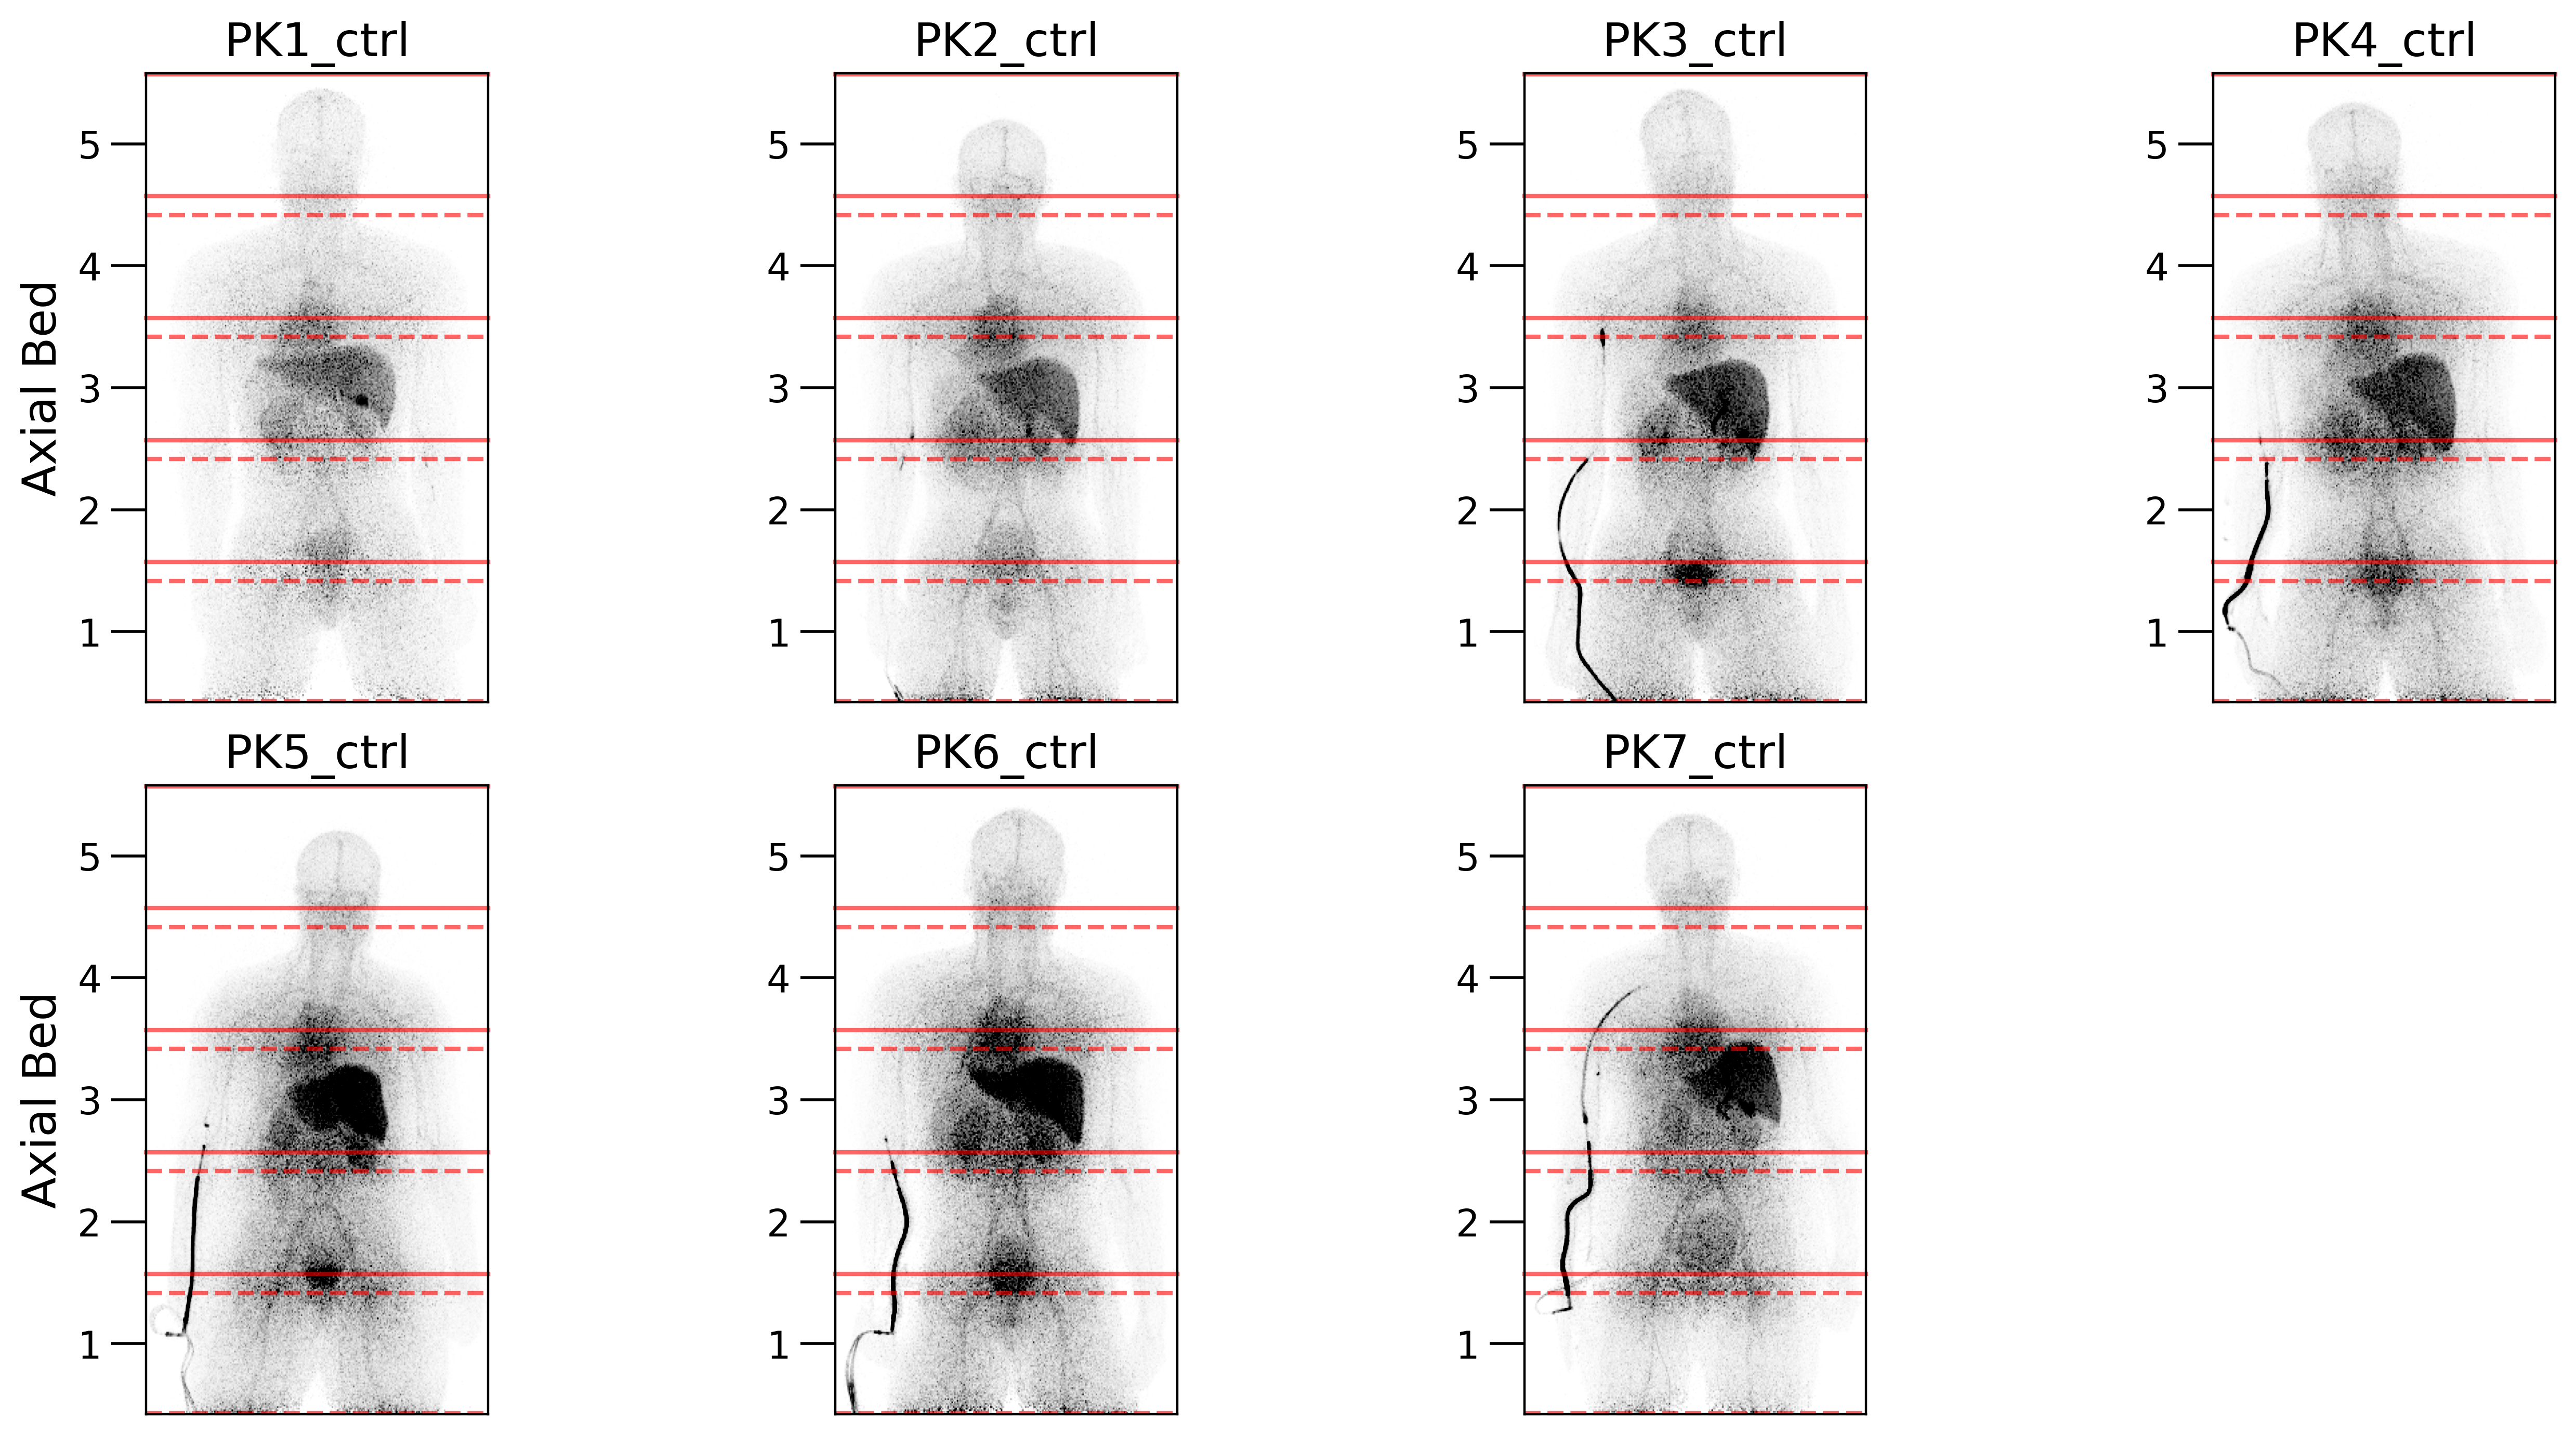
\includegraphics[scale=0.5,angle=0]{3_Results/3_1_DWB_Optimization/figures/3_1_MIPS_ctrl.pdf}
\caption{MIP projections of 7 volunteer control DWB scans with overlay of axial bed start and end location.} 
%TODO: Add over-scan in the CBM D-WB protocols. 
\label{fig3_1:ctrl_mips}
\end{figure}
%
\begin{figure} [ht!]
\centering
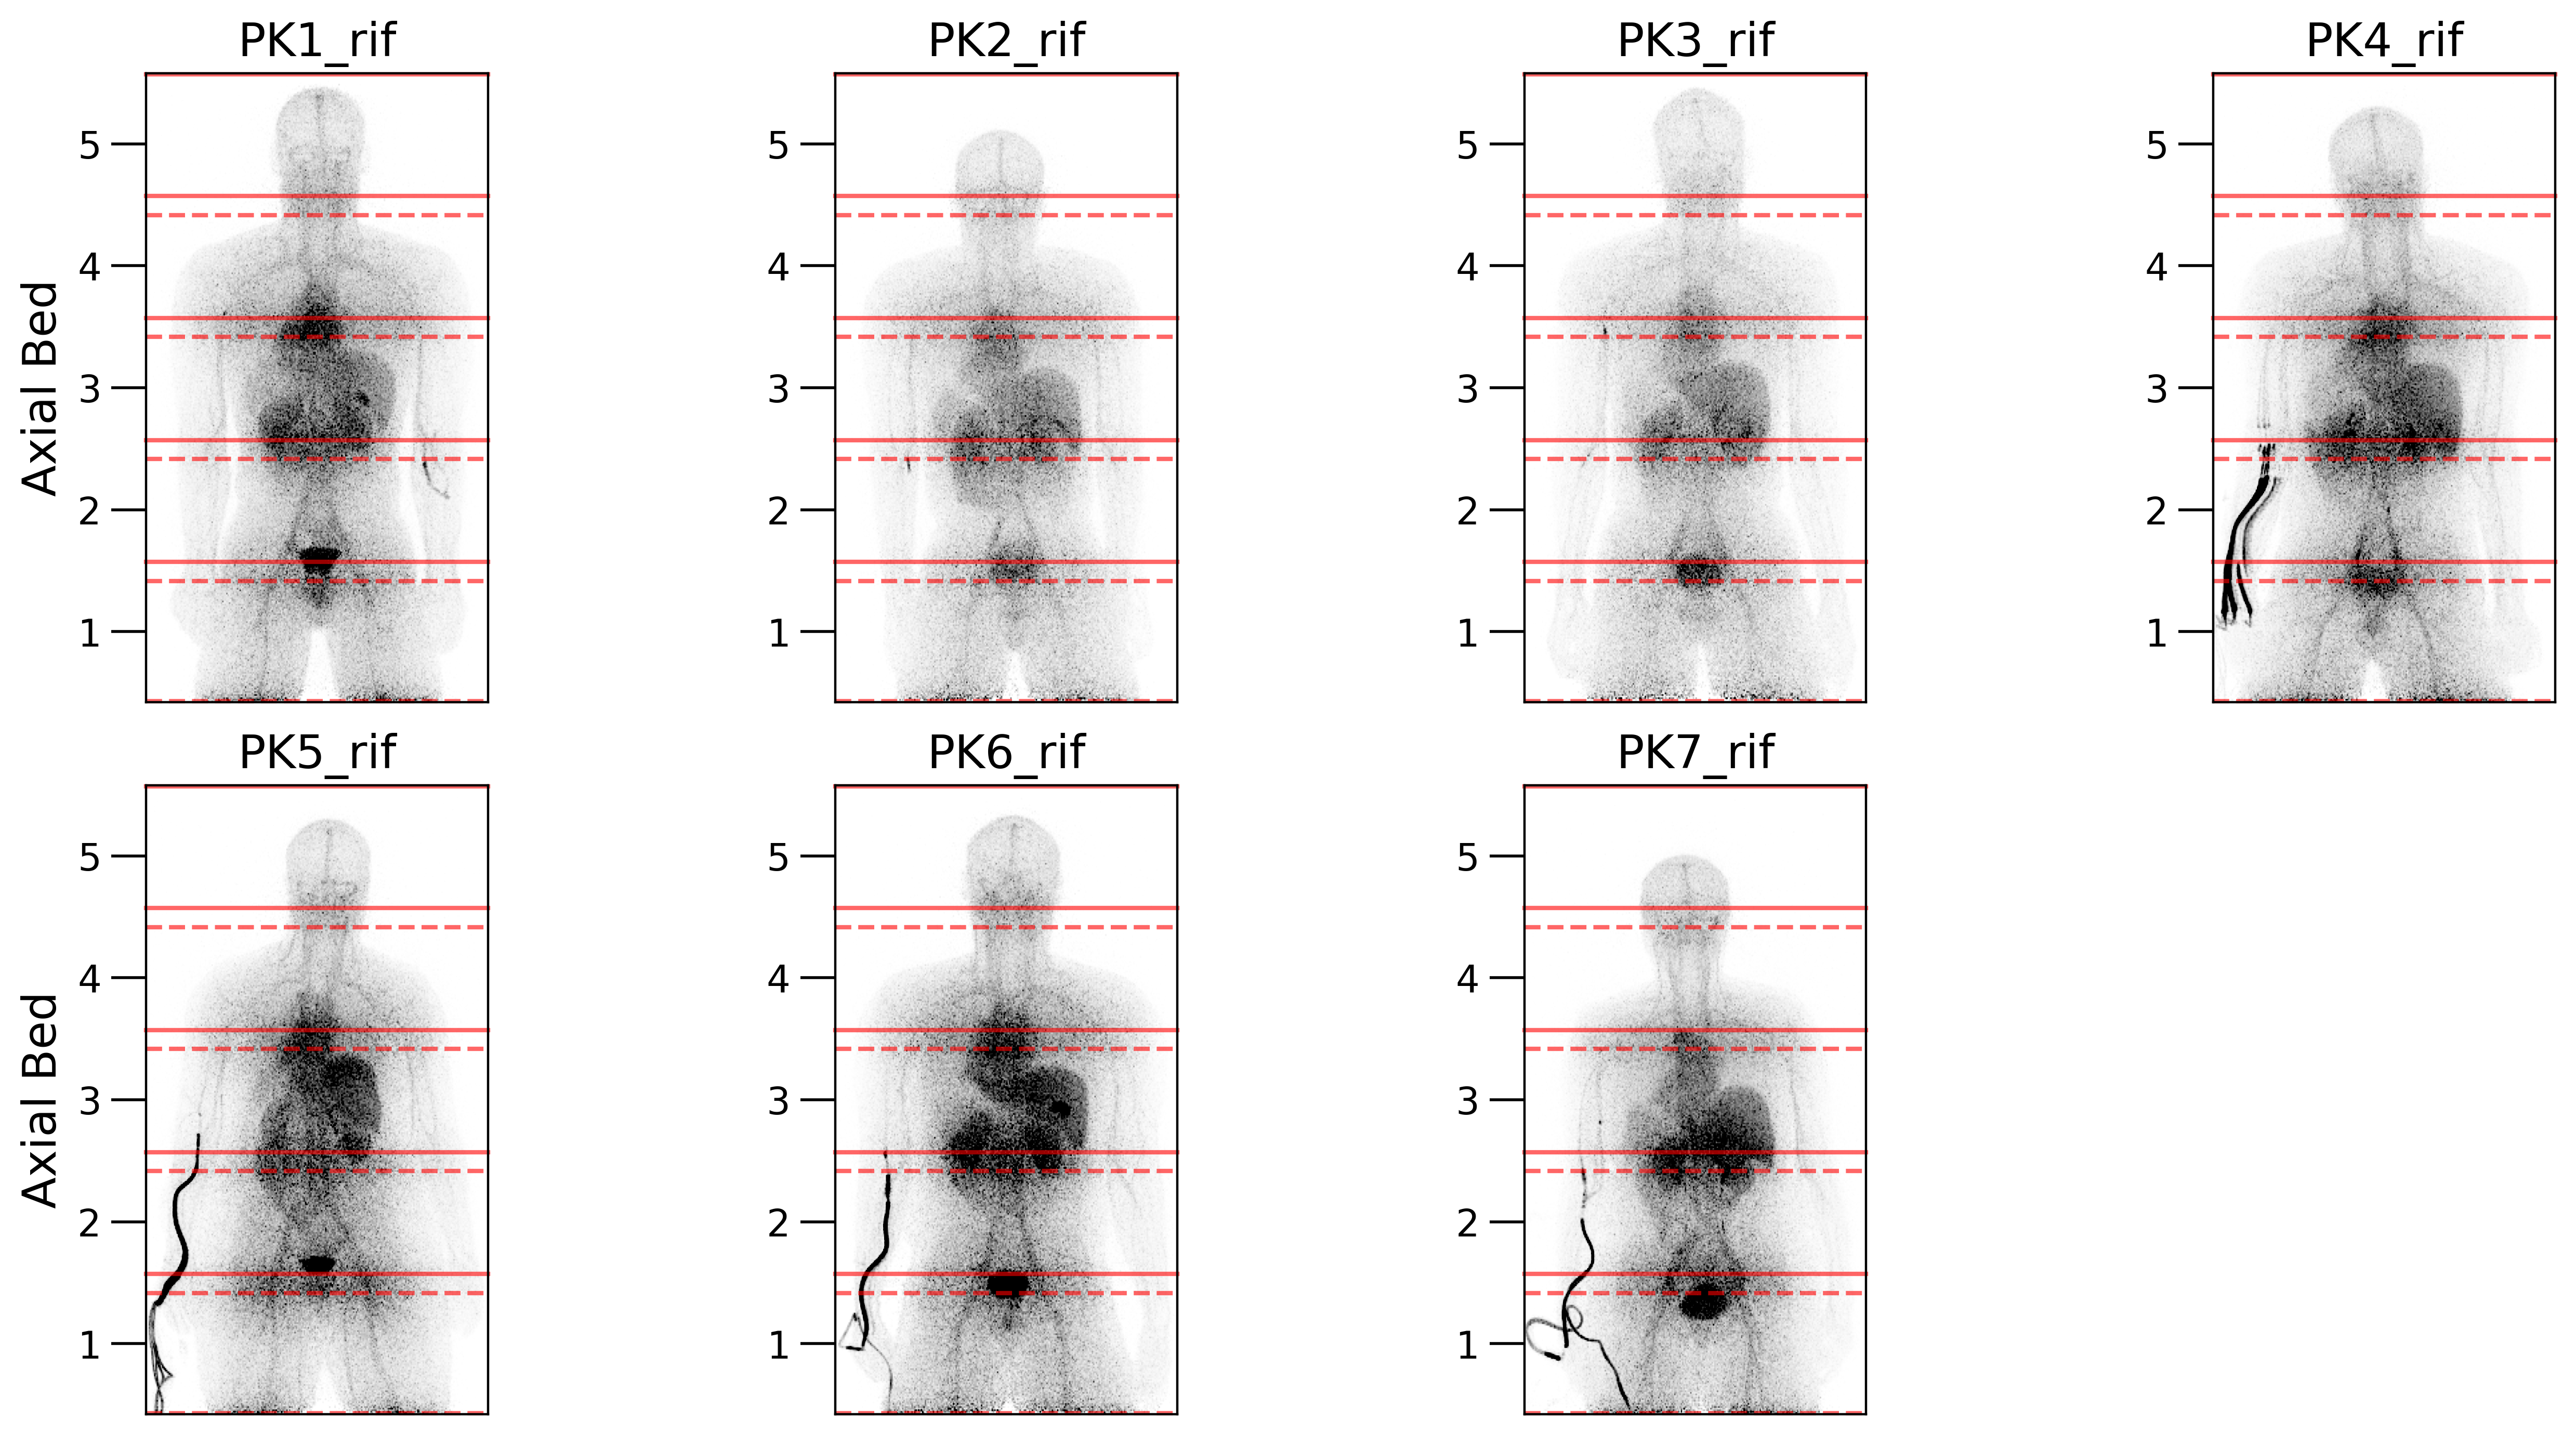
\includegraphics[scale=0.5,angle=0]{3_Results/3_1_DWB_Optimization/figures/3_1_MIPS_rif.pdf}
\caption{MIP projections of 7 volunteer rif DWB scans with overlay of axial bed start and end location.} 
%TODO: Add over-scan in the CBM DWB protocols. 
\label{fig3_1:rif_mips}
\end{figure}
%
%
%
\begin{figure} [ht!]
\centering
\includegraphics[scale=0.5,angle=0]{3_Results/3_1_DWB_Optimization/figures/3_1_BoxPlots_DTBeds.pdf}
\caption{Box plots of intra-bed delays $dl_{bed}$ of the IsotoPK DWB protocol used in practice.} 
%TODO: Add over-scan in the CBM D-WB protocols. 
\label{fig3_1:BoxPlots_beds}
\end{figure}
%
\begin{figure} [ht!]
\centering
\includegraphics[scale=0.5,angle=0]{3_Results/3_1_DWB_Optimization/figures/3_1_BoxPlots_DTSweeps.pdf}
\caption{Box plots of delay between WB Sweeps $dl_{Sweep}$ of the IsotoPK DWB protocol used in practice.}
%TODO: Add over-scan in the CBM D-WB protocols. 
\label{fig3_1:BoxPlots_sweeps}
\end{figure}
%
%
%
\section{Optimization of DWB acquisition protocol on the Signa PET-MR}
Part of this PhD project was allocated in developing a fully-automated DWB protocol on the Signa PET/MR. 
The main requirement for the envisioned protocol was to allow for continuous capture of PET data during DWB acquisition, into a single list-mode file for all bed positions. Then the data could be processed after acquisition, split to individual data for each bed position and reconstructed with the correct bed positional information. Using such an acquisition strategy the delays between bed positions and WB sweeps could be reduced to the time taken by the physical motion of the scanner table alone. 

Towards this goal, the PhD project schedule included a four week industrial secondment with GE healthcare, for the purpose of exploring tools that could enable the automation of DWB protocols. Three weeks of this secondment were spend at factory facilities of GE healthcare (Waukesha, Wisconsin, USA), %with the opportunity the gain insights on the operations of the Signa PET-MR scanner. 
There with help of the PET/MR team it was made possible to exploit in-build factory tools of the Signa PET/MR for the purposes of DWB automation. The two key tools necessary were: 
\begin{itemize}
    \item\textbf{Table Emulation} \\
    This tool allows for disassociation of the table position between the MR and PET system. It is the key tool that allows for the PET system to acquire continuously, while the MR system governs table motion. The disadvantage of this functionality is that once table emulation is enabled MR acquisitions cannot be performed while acquiring PET data.
    \item\textbf{Table Motion} \\
    This tool commands the MR system to execute movements of the scanner bed. It can be used to drive the bed to a target location at a desired speed. 
\end{itemize}

The automated DWB protocol was implemented as a Python class, because the python programming language is available on the PET/MR system's console and allowed for easy integration of the system tools with our designed routines, all under a common system clock for accurate timing of bed movements and registration of events.
The protocol was named "Auto-IsotoPK", but despite its name is a generic DWB protocol that is not limited to the IsotoPK pharmacokinetic study. It allows for an optional single-bed dynamic phase to be acquired before starting the DWB acquisition. It also allows for any number of beds to be used for DWB acquisition and positioning of the beds using for each examination using an initial MR scout image. 
Because MR acquisitions cannot be performed after \textit{Table Emulation} is enabled, all bed position MRACs must be acquired prior to the PET examination and used for all WB sweeps of the study.

A short \gls{sop} on the operation of the protocol is given in Appendix~\ref{chap:AppendixA}.

After the procedure is completed, the whole PET study is stored as a single list-mode file. The precise timing information of the acquired bed positions are saved in a log file, to be used for the post-processing procedure. 

\subsection{Results from NHP study}
After initial tests using phantoms, the protocol was tested on an actual pre-clinical DWB study. A macaque was scanned under full sedation with a novel $^{18}$F-Crizotinib tracer, that was being investigated for uses with \gls{nsclc}. The DWB study was required to examine tracer crossing of the blood-brain barrier and tracer uptake and excretion from other organs. The macaque was injected with 185 \si{\mega \becquerel} of the novel tracer. An initial dynamic phase was requested, centred over the brain for a duration of 90 s, followed by a DWB study of 3 bed positions. The study was planned for an approximate total duration of one hour. A total of 28 WB sweeps and frames per bed were fitted in the study, with the framing of 3$\times$10~\si{\s}, 5$\times$20~\si{\s}, 5$\times$30~\si{\s}, 5$\times$45~\si{\s}, 10$\times$60~\si{\s}. 
Acquisition of the required MRACs was performed prior to injection, at the planned bed positions shown in figure~\ref{fig3_1:Macaque_MRI}. In this acquisition only the body coils of the PET-MR system were used, designed for use with the human body size and load, which resulted in sub-optimal MR quality for automated estimation of attenuation maps. Attenuation maps had to be created manually in post-processing of the data to adequately correct the PET reconstruction for attenuation.  

\begin{figure} [ht!]
\centering
\includegraphics[scale=0.5,angle=0]{3_Results/3_1_DWB_Optimization/figures/3_1_Macaque_MRI.pdf}
\caption{MRAC acquisitions of NHP study showing the planned bed positions of the two acquisition phases.}
\label{fig3_1:Macaque_MRI}
\end{figure}

Following the MRAC acquisitions and after the automated acquisition protocol, the study started with the injection of the NHP subject followed by an hour of PET imaging. 
The complete study dataset was recorded in a single list-mode file, of which the head curve (curve of prompts rate with time) can be seen in figure~\ref{fig3_1:Macaque_Head_Curve}. By overlaying the recorded timing information over this curve, the two phases of the acquisition (SBD and DWB) as well as the three bed position of the DWB acquisition can be distinguished. The initial 260 second of the recorded list-data's head curve with the overlaid phases and bed positions are shown in figure~\ref{fig3_1:Macaque_Head_Curve_Phases}. 

\begin{figure} [ht!]
\centering
\includegraphics[scale=0.45,angle=0]{3_Results/3_1_DWB_Optimization/figures/3_1_Macaque_Head_Curve.pdf}
\caption{Head curve (prompts rate against time) of the acquired NHP study DWB data in a single list-mode file using the optimised protocol.}
\label{fig3_1:Macaque_Head_Curve}
\end{figure}

\begin{figure} [ht!]
\centering
\includegraphics[scale=0.45,angle=0]{3_Results/3_1_DWB_Optimization/figures/3_1_Macaque_Head_curve_Phases.pdf}
\caption{Head curve (prompts rate against time) of the acquired NHP study showing the SBD and DWB phases of the acquisition and the three DWB bed positions.}
\label{fig3_1:Macaque_Head_Curve_Phases}
\end{figure}
%
Using the timing information recorded by in the log file, the data were split into four individual bed position datasets and were processed with the GE-PET toolbox individually as single bed dynamic studies. The list-mode data along with the generated corrections were then exported into the CASToR data-file format for subsequent reconstruction tests. A \gls{mip} view of 3D reconstructions (averaged across all dynamic frames) is shown in figure~\ref{fig3_1:Macaque_PET}. \\
An image derived input function was estimated from the PET data using the right carotid VOI, which was visible on both phases of the acquisition, and the left ventricle. Both VOIs provided similar blood activity values in the DWB phase and were averaged to produce the final IDIF.
%
\begin{figure} [ht!]
\centering
\includegraphics[scale=0.45,angle=0]{3_Results/3_1_DWB_Optimization/figures/3_1_Macaque_PET.pdf}
\caption{MIP views of the NHP study's reconstructed PET images, for the two phases of the acquisition.}
\label{fig3_1:Macaque_PET}
\end{figure}
%
%
\begin{figure} [ht!]
\centering
\includegraphics[scale=0.45,angle=0]{3_Results/3_1_DWB_Optimization/figures/3_1_NHP_InputFunction.pdf}
\caption{NHP study's image derived input function using information from multiple bed positions.}
\label{fig3_1:Macaque_PET}
\end{figure}
%
Using the log timing information an estimation of the delays (time gaps) for this single NHP study using the automated acquisition protocol was made. The results showed an average intra-bed delay time $dl_{bed}$ of 3.77 s (95\%CI: 3.62,3.91) and an average delay time between sweeps $dl_{Sweep}$ of 4.6 s (95\%CI: 4.53, 4.67).


\section{Discussion}

Furthermore the hard-set bed positions do not always allow for optimum use of the effective A-FOV in each examination, as seen for example in examination PK2 in figures~\ref{fig3_1:ctrl_mips}~and~\ref{fig3_1:rif_mips}. In some cases a fewer number of bed positions might be adequate and preferable as it would lead to substantial increase of sampling frequency per bed. \\




\section{Conclusion}



%\subsection{Auto-IsotoPK: Continuous Bed Motion on the Signa PET-MR}
%The flexibility offered by the use of the automated protocol and the dedicated \"Table Motion\" tool allowed for testing the proof of concept of CBM on the Signa PET-MR scanner. Although this acquisition mode is not supported by the system, we emulated the acquisition of a single whole-body sweep by commanding a table movement at a speed of \SI{5}{\milli\metre\per\second}. The duration of the total sweep, that covered the three bed positions that were acquired in the previous DWB study and included an 50\% overscan, was ...

\iffalse
\section{Implementation of dynamic functions in CASToR }
How dynamic reconstruction was implemented in CASToR (in relation to the methods explained in the theory section). \\

\section{Simulation Study}
The gap paper and expand. Describe more on spectral model and do $K1$ and spectrum comparisons also. \\

\section{Advancements in WB and WB-Dynamic reconstruction}
All the déjà unique implementations in CASTOR. \\
Theory and practice for Dynamic Whole Body reconstruction (direct and nested), with toy simulation example and macaque data. \\

\section{Real exam data: IsotoPK, Lung NSCLC etc.}
All the works with real data , single and multi bed.  \\ 
The use of the Spectral model advantages in pharmacokinetic studies. \\

\section{Other projects: HYBRID, CASToR etc.}
All the other projects within Hybrid ! \\
Laura's Simulation & CNN \\
Lalith's MoCo mMR Brain GAN.
\fi